\begin{frame}
\frametitle{\insertsection} 
\framesubtitle{\insertsubsection}
Рассмотрим в качестве примера вызов:
\inputminted{java}{code/FlatMapFactorizeExample.java}
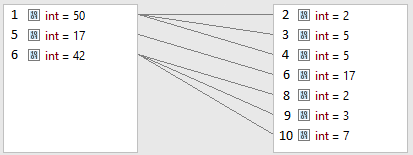
\includegraphics[scale=0.8]{img/flatMapExample.png}

Решая такие же задачи и для остальных методов, получим для них отображение. Такой подход работает почти для всех методов. Исключение - операции с состоянием. Для них можно придумать отдельное решение.
\end{frame}
